\if 10
\newpage
\subsection{Solutions to selected exercises}

\medskip
\noindent Solution~\ref{ex:A1}:\\
One possible regular expression would be $(a|b|\epsilon)b(ab)^*(b|\epsilon)$.

\medskip
\noindent Solution~\ref{ex:A2}:\\
 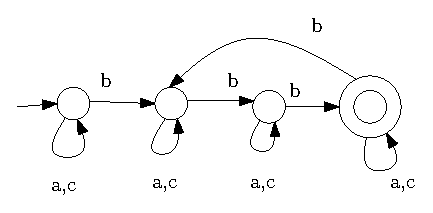
\includegraphics{figs/automata3k_b.eps}

\medskip
\noindent Solution~\ref{ex:Aprime}:\\
Since there are an infinite number of prime numbers, any DFA that
accepts this language must have at least one cycle formed by transitions
via the character 0.  Let $k$ be the length of one such reachable cycle.
Let $x$ be a string that lands on an accepting state on this cycle 
(that is, $x$ has a prime number of 0's).  Any string $x0^k$ is also accepted 
by the DFA.  This shows that the number of primes less than $n$, as $n$ 
approaches $\infty$, is $O(n/k)$.  This contradicts the Prime Number 
Theorem: The number of primes less then $n$, $\Theta(n)$, is proportional 
to $\ln(n)$.  [that is, $\lim_{n \rightarrow \infty } \Theta(n) / ln(n) = 1$ ]

\medskip
\noindent Solution~\ref{ex:A3}:\\
Minimum length distinguishers for several pairs of states $s_1$ and $s_2$ 
are given in the following table.\\
\def\inclans{1}
\begin{minipage}{\textwidth}
\setlength\tabcolsep{16pt}
\setlength\arrayrulewidth{.5pt}
%\renewcommand{\baselinestretch}{1.5}\large\normalsize
        \begin{tabular}{|c|c|c|}
        \hline
        State $s_1$ & State $s_2$ & \hspace*{2cm} Distinguisher
\hspace*{2cm}  \\   \hline
        0 & 1 & \ifnum\inclans=1{$a$} (or $b$)\fi \\
        \hline
        0 & 5 & \ifnum\inclans=1{$aa$} (or others of length 2)\fi \\
        \hline
        1 & 2 & \ifnum\inclans=1{N/A}\fi \\
        \hline
        1 & 3 & \ifnum\inclans=1{$\epsilon$}\fi \\
        \hline
        3 & 4 & \ifnum\inclans=1{$a$} (or $b$)\fi \\
        \hline
        \end{tabular}
\end{minipage}

\medskip
\noindent Solution~\ref{ex:A4}:\\
%\begin{proof}
Assume a DFA machine $M$ with $m$ states accepts $L=\{0^n1^{2n}
\mid n \geq 0\}$.  Consider what states the machine $M$ reaches with
each of the following strings $x_1=0$, $x_2=00$, \ldots, $x_m=0^m$,
$x_{m+1}=0^{m+1}$.  Since $M$ has only $m$ states there must be
two strings $x_i$ and $x_j$ ($i\not=j$) that reach the same state.
Now consider the two strings $0^i1^{2i}$ and $0^j1^{2i}$.  The machine
$M$ must accept both (or neither).  Thus $M$ does not accept $L$.
The same argument holds for any finite state machine.
%\end{proof}


\medskip
\noindent Solution~\ref{ex:A5}:\\
There are two common ways to build an automaton for the
intersection of
two regular languages $L_1$ and $L_2$ that are accepted by DFA $M_1$ and
$M_2$, respectively.

Method 1: Build a new automaton $M$, where the states $Q$ are $Q_1
\times Q_2$.  Accepting states $(q_1,q_2) \in Q$ if and only if
$q_1$ and $q_2$ are accepting states of $M_1$ and $M_2$. Transitions
$\delta((q_1,q_2),c)=(q'_1,q'_2)$ if and only if $\delta_1(q_1,c)=q'_1$
and $\delta_2(q_2,c)=q'_2$. The unique starting state is $(s_1,s_2)$
where $s_1$ and $s_2$ are the start states for $M_1$ and $M_2$,
respectively.

Method 2: Use set theory fact that $L_1 \cap L_2 =
\overline{\overline{L_1} \cup \overline{L_2}}$, where $\overline{L} =
\Sigma^* \setminus L$.  We construct an automaton $M'$ for
$\overline{L}$ by taking a DFA $M$ for $L$ and changing accept
states to non-accept states (and non-accept states to accept states).

\medskip
\noindent Solution~\ref{ex:diff}:\\
First note that $L_2 \setminus L_1 = L_2 \cap \overline{L_1} =
\overline{\overline{L_2} \cup L_1}$.  Then do the following. \\
1. Build DFA $M_3$ for $\overline{L_2}$.  (swap accept/reject states) \\
2. Build NFA $M_4$ for $\overline{L_2} \cup L_1$.  \\
3. Convert $M_4$ to DFA $M_5$.\\
4. Build DFA $M$ from $M_5$. (swap accept/reject states)

\medskip
\noindent Solution~\ref{ex:even}:\\
Use something like: $0\mid1(0\mid1){}^*0$

\medskip
\noindent Solution~\ref{ex:nfaclosure}:\\
One possible answer is:\\
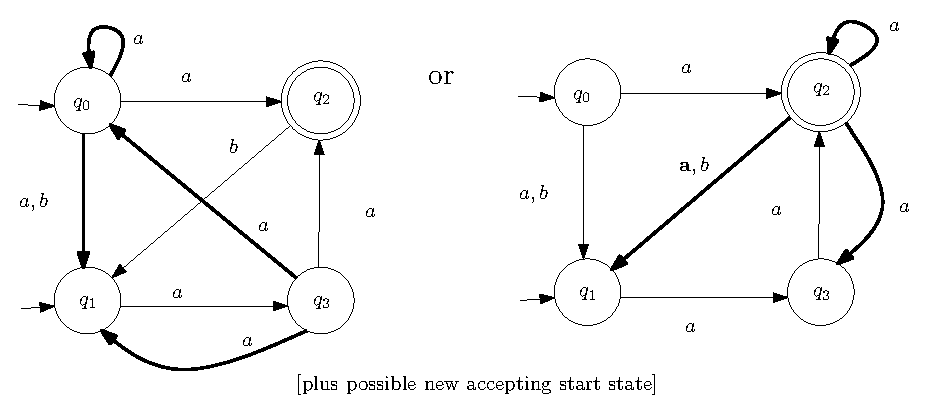
\includegraphics[width=3.8in]{figs/NFAforClosureAns}

\medskip
\begin{samepage}
\noindent Solution~\ref{ex:nfaconcat}:\\
Two possible solutions are:\\
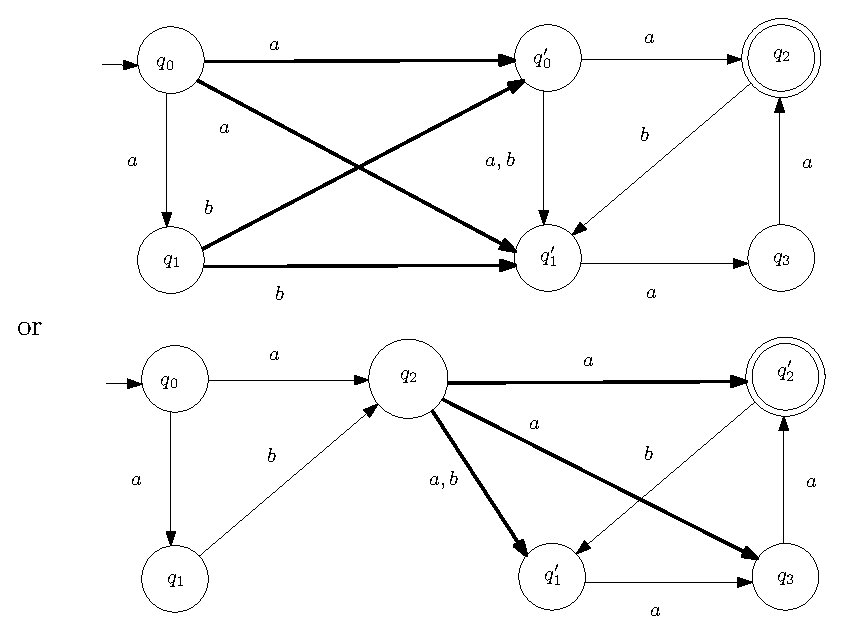
\includegraphics[width=3.5in]{figs/NFAforConcatAns}
\end{samepage}

\fi % solution section
